\documentclass[a4paper,11pt,titlepage]{article}
\usepackage{graphicx}
\author{Abrie Greeff\\B.Sc Hons (Computer Science)\\Department of Computer Science\\University of Stellenbosch\\Supervisor:\\Dr. L van Zijl}

\title{Hand Motion Detection From Video Data}

\begin{document}
\maketitle
\tableofcontents
\newpage
\section{Introduction}
\newpage
\section{Requirements Engineering and Specification}
\subsection{Description of Requirements}
This project is a part of the South African Sign Language (SASL) dictionary initiative. The purpose of this project is to obtain motion data from a set of videos and translate hand movements into two-dimensional Cartesian coordinates.

\subsection{Informal Specification}
The user will provide a Mpeg 2 video file as input. This video will contain one or more gestures that is each related to a word in the SASL. The first application developed for this project will inspect this video data and split the data into smaller video files each corresponding to a different gesture.

The second application developed for this project will handle the retrieval of the Cartesian coordinates of the hand movements from the smaller video data files. These hand movements will be stored in a file with the corresponding word associated with this gesture. The process of extracting the information from the videos will be autonomous.

\newpage
\section{Formal Specification}
The formal specification will formally specify the requirements for each component of the project.

\subsection{User Interface}
The user interface for the project must be a graphical user interface (GUI). The GUI must support the playing of Mpeg 2 videos. The video file name is specified by the user. If the application is unable to load the video data a suitable error message must be displayed. The tracking of movement in the video data can be specified as an action that the user selects or can be done when the video is loaded.

The GUI must allow the user to specify what the gesture, associated with the hand movements in the video, is in SASL. This is necessary to make sure the correct word is associated with the correct hand gestures. If the application is unable to extract enough information to do correct hand tracking a suitable error message must be displayed to indicate a problem.

The application only needs to execute on a Linux operating system. If a video is loaded that may take up all the system memory the user must be notified that he or she does not have enough system memory. The application must support videos of different sizes.

\subsection{Video Data}
A video is a set of chronological frames. Each frame is a picture and when played together they form the video. A video file can also contain audio data. For the purposes of this project audio data will be ignored because we are only interested in the video motion.

Each frame has the same dimensions, width and height. Every set of non-negative integer coordinates in this two-dimensional plane points to a picture element (pixel). Every pixel represents a colour value. In general all colour values have three 8-bit components, called the red, green and blue (RGB) values. When the intensities of these components are changed different colours can be formed.

For the purpose of this project it can be assumed that all video files will be of the same format and contain similar data. This means that it can be assumed that all videos will have a single person standing approximately in the middle of the picture. This person will perform one or more hand gestures that are associated with words in SASL.

The video format that must be supported is the Mpeg 2 format. Videos will be loaded into memory before processing, therefore it is neccessary to determine what the size of videos are and if the application is able to handle it. The colour of the pixels in the video frames may be colour or greyscale pictures. It may be assumed that all videos will be recorded from a static camera. The application must however have a small level of compensation for cameras that are not static.

\subsection{Human Body Features}
We are interested in the body proportions of an average human. From Wikipedia \cite{wiki} we obtain the following proportions.
The average human is 7 to 7.5 average head lengths tall. The pubis is at mid-height of the average human. The lower arm is one and a $1 \over 4$ heads long and the average hand is $3 \over 4$ heads long. If we look at Da Vinci's Vitruvian Man (see Fig. \ref{Fig:vitruvian}) we can examine these proportions.
\begin{figure}[htbp]
   \centering
   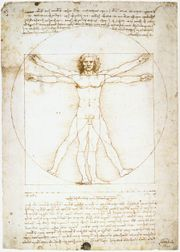
\includegraphics[width=4cm]{Vitruvian.png}
   \caption{Virtuvian Man}
   \label{Fig:vitruvian}
\end{figure}

The application must be able to handle data from average humans. It does not matter what the race or sex of the person is. The length of the person must be relatively average. This is to ensure that the proportions are correct.

\subsubsection{Head}
The human head is situated at the center of the human body if we are viewing a human from the front. The head is situated on top of the shoulders. If a person is standing in a relaxed upright position with their arms pointing downwards the head will be the highest position of the body.

\subsubsection{Elbows}
The elbows are the connection between the upper and lower arms. If a person is standing in a relaxed upright position with the arms pointing downwards the elbows will be situated roughly halfway between the hands and the shoulders. The upper arm connects the elbow with the shoulder and the lower arm connects the elbow to the hand.

\subsubsection{Hands}
As defined in the previous subsection a hand is connected to the elbow by the lower arm.

\subsection{Video Noise}
Most videos that are commercially available today have some form of data compression to decrease the size of the video data. There are two types of data compression. Lossless data compression is when data is compressed and the uncompressed data is exactly the same as the original. Unfortunately most video data compression algorithms uses lossy quality compression. This is when the uncompressed data is not the exactly the same as the original, but looks the same to the human eye.

This leads to a problem called video noise. Video noise are different between videos and also each subsequent frame in a video. When a video has the same background for every frame in the video it is possible to eliminate most of the noise in the video. This is because most noise is only small fluctuations in the values of the RGB components.

To eliminate this noise a filter needs to be applied on the data. This filter needs a small value called a threshold to indicate how much fluctuation is allowed in the RGB components of every pixel between each frame. This value must not be too high because we must still be able to decide if there is a fluctuation in the data or if there were motion between the two frames.

\subsection{Data Extraction}
The most important aspects of this project is extracting the correct data from the video files, while still having an autonomous system. Therefore we need to extract the correct information from the video files. We are interested in the hand gestures and thus we must find a way to extract the movement of the hands from the video frames. If we are able to extract the hands in the first frame and follow the movements of the hands in the subsequent frames we will succeed in our goals. The following subsections focuses on finding the hands in the first frame and the next section on tracking the movements of the hand.

\subsubsection{Edge Detection}
Edge detection is the detection of movements between frames. This is called edge detection because the movements is picked up at the edges of areas where objects move over other objects.

In the case of human movement this enables us to pick up areas that may have previously contained a human body part. We find these areas by applying a threshold value. If a value is over this threshold we can assume movement occurred.

Movements between two frames are not enough to determine the outline of a human body. Therefore we need to find the mean and standard deviation of all the RGB components of each detected edge in the entire video. The mean $\mu$ and standard deviation $\sigma$ is calculated as
\begin{displaymath}
{X_{i,j}} =
\Bigg{\lbrace} \begin{array}{ccc}
Rgb_{i,j} & & when\;Rgb_{i,j} \geq thres \\
0 & & when\;Rgb_{i,j} < thres
\end{array} 
\end{displaymath}
\begin{displaymath}
n = amount\; of\; pixels\; over\; threshold
\end{displaymath}
\begin{displaymath}
\mu = \frac{1}{n} \sum_{i=0}^{w-1}\sum_{j=0}^{h-1} X_{i,j}
\end{displaymath}
\begin{displaymath}
\sigma^2 = \frac{1}{n - 1} \sum_{i=0}^{w-1}\sum_{j=0}^{h-1} (X_{i,j} - \mu)^2
\end{displaymath}
\begin{displaymath}
\sigma = \sqrt{\sigma^2}
\end{displaymath}

If we now apply a simple test
\begin{displaymath}
\mu - 0.3*\sigma < RGB(i,j)
\end{displaymath}
we are able to find the edges in every frame with high accuracy. If we examine the equation we can see that we look at the mean RGB value at each pixel and allow a small fraction of deviation from the mean.

\subsubsection{Body Part Isolation}
The edges does not give enough information of the human body parts to successfully track movement. We now need to determine from the edges in the first frame where the head, elbows and hands are. The first frame is inspected because all movement starts from there. Furthermore it can be assumed that the video data used in this project will always have a first frame where the person is standing upright, with the elbows below the head and the hands below the elbows.

This assumption makes it possible to isolate certain body parts. We want to isolate the head because in later frames it may happen that a hand passes over the face. If this happens we want a estimate of what area the head is contained in. If we take our assumptions and the information from Section 3.3 into account we can find the head in the center of the upper half of the first frame. We must check the edges to find the correct position.

Once we have found the head we must find the elbows and hands. From the assumption that the person is standing in a relaxed upright position we can find the center line of the body thus allowing us to calculate the left and right hand sides of the body.

We know the elbows are above the hands and if we look at the highest edges on the left and right of the center line we will find the relative positions of the two elbows.

The hands are isolated basically the same way as the elbows. The difference is that we now know that they are situated at the bottom of the frame. Again a search is conducted for the best fit for the left and right hands. Because we have defined a center line for the body it does not matter if the hands are folded because the relative positions will still be computed.
\subsubsection{Skin Tone Selection}
The skin tone is the last important detail we need. Together with the edges it will enable us to successfully find body detail in each frame. To compute the skin tone we need the mean and standard deviation of the RGB components of the lower arm. From the body parts isolated from the previous subsection we are able to roughly determine a linear equation for each lower arm. By testing coordinates against this equation the mean and standard deviation of the lower arms can be computed.

\subsection{Hand Movement Tracking}
From the previous section we have enough information to accurately determine the inner and outer edges of the lower arms and the head. By applying an image mask the head can be removed from each frame thus leaving only the arms in every frame.

By applying a least squares algorithm between every frame we can track the movement of the arms. Because only tracking single pixels can lead to incorrect tracking we need to track the areas that are defined to be the elbows and hands. We need the elbows because we know what the relative offset of the hands from the elbows are.
\subsection{Output Coordinates}
The output coordinates of the tracking of the hands can not be the same coordinates as the video coordinates. This is because different videos have different dimensions. The coordinates must be relative to the size of the head as well as the position of the center of the head.
\section{Prototypes and Design}
\section{Testing}
\section{Future Work}

\begin{thebibliography}{9}
\bibitem{wiki} Wikipedia, the free encyclopedia,
\emph{Body Proportions - Wikipedia, the free encyclopedia},	
[Online], Available from \emph{http://en.wikipedia.org/wiki/Body\_proportions.htm}
\end{thebibliography}
\end{document}
